\section{Motivation}
\label{sec:motivation}

Consider how we might implement a highly available bank account on top of an
eventually consistent data store, with the \emph{integrity} constraint that the
balance should never drop below 0. We will begin by implementing the bank
account replicated data type (RDT) in \name, and then describe the mechanisms
to obtain the desired correctness guarantees.

\subsection{RDT specification}

A key novelty of \name is that it allows the addition of new RDTs to the
store, greatly improving programmability.  Specifically, programmers no
longer have to coerce application logic to conform to to store-provided data
types. In addition, \name treats the convergence semantics of the data type
separately from consistency properties. This separation of concerns allows
the programmer to \emph{operationally} reason about conflict resolution,
while permitting \emph{declarative} reasoning for consistency. As mentioned
in the previous section, RDTs are described in terms of operations on a RDT
object, where each operation is described as a reduction over the state of
the object i.e., the list of effects.

Assume that the bank account object provides three operations: \cf{deposit},
\cf{withdraw} and \cf{getBalance}, with the assumption that the \cf{withdraw}
fails if the account has insufficient balance.  Every operation in \name is
of the following type, written in Haskell syntax:

\begin{codehaskell}
type Operation = (Effect e, Arg a, Res r)
               => [e] -> a -> (r, Maybe e)
\end{codehaskell}

\noindent An operation takes a list of effects (the \emph{context} for the operation), an
argument and returns a result along with an optional effect. Read-only
operations do not return any effect. If an effect is returned, it is added to
the state of the object at the current replica, and asynchronously sent to
other replicas. The implementation of the bank account operations in \name is
given below:

\begin{codehaskell}
data Acc = Deposit_ Int | Withdraw_ Int
				 | GetBalance_

getBalance :: [Acc] -> () -> (Int, Maybe Acc)
getBalance ctxt _ =
  let res = sum [x | Deposit x <- ctxt]
          - sum [x | Withdraw x <- ctxt]
	in (res, Nothing)

deposit :: [Acc] -> Int -> ((), Maybe Acc)
deposit _ amt = (amt, Just $ Deposit_ amt)

withdraw :: [Acc] -> Int -> (Bool, Maybe Acc)
withdraw ctxt v =
	if sel1 $ getBalance ctxt () >= v
  then (True, Just $ Withdraw_ v)
	else (False, Nothing)

mkOperName ''Acc
\end{codehaskell}

The datatype \cf{Acc} represents the effect type for the bank account. The
context of the operations is a snapshot of the state of the object at some
replica. In this sense, every operation on the RDT is atomic, and thus
permitting sequential reasoning for implementing eventually consistent data
types. We have implemented a large corpus of RDTs for realistic benchmarks
including shopping carts, auction and micro-blogging sites in few tens of lines
of code.

The last line in the above code snippet uses Template Haskell~\cite{} to
generate the following datatype declaration:

\begin{codehaskell}
data OperName = Deposit | Withdraw | GetBalance
\end{codehaskell}

\noindent that declares a nullary constructor for each of the constructors in
the given type, dropping the tailing underscore from the original constructor
names. This declaration will come in handy for writing the contracts.

\subsection{Anomalies under Eventual Consistency}

Our goal is to choose the correct consistency level for each of the bank
account operations such that (1) the balance never drops below zero and (2) the
\cf{getBalance} operation never incorrectly returns a negative balance. To be
able to do this, we need to consider the anomalies that could arise under
eventual consistency.

\begin{figure}
\centering
\subfigure[Unsafe withdraw]{\label{fig:unsafeWithdrawAnomaly}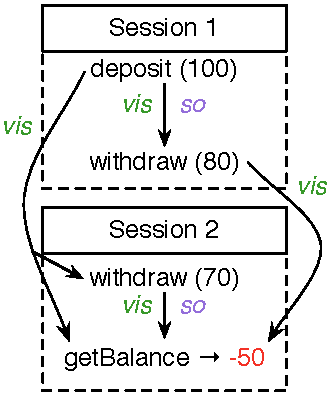
\includegraphics[width=0.34\columnwidth]{Figures/Motivation4}}
\hfill
\subfigure[Negative balance]{\label{fig:negativeBalanceAnomaly}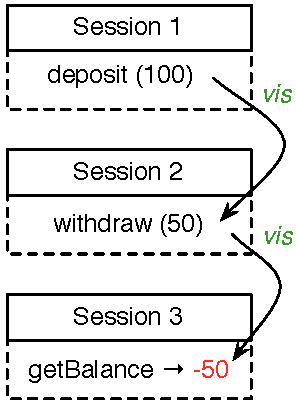
\includegraphics[width=0.31\columnwidth]{Figures/Motivation2}}
\hfill
\subfigure[Missing update]{\label{fig:missingUpdateAnomaly}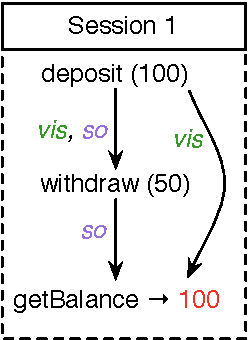
\includegraphics[width=0.26\columnwidth]{Figures/Motivation1}}
\caption{Anomalies possible under eventual consistency for the get balance operation.}
\label{fig:cleanliness_examples}
\end{figure}

Consider the execution shown in Figure~\ref{fig:unsafeWithdrawAnomaly}. Assume
that all operations in the figure are on the same bank account object with the
initial balance being zero. Session 1 performs a \cf{deposit} of 100, followed
by a \cf{withdraw} of 80 in the same session. The \cf{withdraw} operation
witnesses the deposit and succeeds\footnote{Although visibility and session
order relations relate effects, we have abused the notation in these examples
to relate operations, with the idea that the relations relate the effect
emitted by those operations}. Subsequently, session 2 perform a \cf{withdraw}
operation, but importantly, due to eventual consistency, only witnesses the
\cf{deposit} from session 1, but not the subsequent withdraw. Hence, this
\cf{withdraw} also \emph{incorrectly} succeeds, violating the integrity
constraint. A subsequent \cf{getBalance} operation, that happens to witness all
the previous operations,  would report a negative balance.

It is easy to see that the only way to ensure the integrity constraint on
\cf{balance} is to prevent concurrent withdrawals on the same bank account
object. This can be done by insisting that \cf{withdraw} be executed with
strong consistency properties. Although this prevents the integrity constraint
from being violated, a strongly consistent \cf{withdraw} itself is not
sufficient to prevent \cf{getBalance} from ever reporting a negative balance to
the end user.

Consider the execution shown in fig.~\ref{fig:negativeBalanceAnomaly}, which
consists of three concurrent sessions performing a \cf{deposit}, a
\cf{withdraw}, and a \cf{getBalance} operation, respectively, on the same bank
account object. As before, assume that the initial balance in the account is
zero. As the \cf{vis} edge indicates, operation \cf{withdraw(50)} in session 2,
can witnesses the effects of \cf{deposit(100)} from session 1, leading it to
rightfully conclude that the current balance is 50. Consequently,
\cf{withdraw(50)} is performed safely. The effect of this \cf{withdraw}
operation subsequently becomes visible to the \cf{getBalance} in Session 3.
However, because \cf{getBalance} only witnesses the effect of the \cf{withdraw}
operation from session 2, but not the \cf{deposit} from session 1, reports the
balance of negative 50 to the user.

Producing a negative balance is not the only inconsistency that the user is
exposed to under an eventually consistent bank account. Figure
~\ref{fig:missingUpdateAnomaly} shows an execution where the \cf{getBalance}
operation in a session does not witness the effects of an earlier \cf{withdraw}
operation performed in the same session, possibly because it was served by a
replica that has not yet merged the \cf{withdraw} effect, served by a different
replica. This anomaly leads the user to incorrectly conclude that the
\cf{withdraw} operation failed to go through.

Although it is easy to understand the reasons behind the occurrence of the
aforementioned negative balance and missing update anomalies, finding the
appropriate fixes is not readily apparent. Making \cf{getBalance} a strongly
consistent operation is definitely sufficient to avert anomalies, but is it
really necessary? Given the cost of enforcing strong
consistency~\cite{DynamoDB, Pileus}, it is preferable to avoid it unless
there are no viable alternatives.  Exploring the space of these alternatives
requires understanding the subtle differences in semantics of various kinds
of weak consistency alternatives.

\subsection{Specifications and Contracts}

\name helps facilitate the mapping of operations to appropriate consistency
levels by letting the programmer declare application-level consistency
constraints as \emph{contracts} that axiomatically specify the set of allowed
executions involving this operation.  In the case of the bank account example,
any execution that does not exhibit the anomalies described in the previous
section is a \emph{well-formed} execution on the bank account object.  By
specifying the set of legal executions for each data type in terms of a trace
of operation invocations on that type, \name\ ensures that all executions over
that type are well-formed.

\begin{figure}
%Careful while adjsting spaces in the following code; screws "::" alignment.
\begin{codehaskell}
data Effect, Rel, Prop, Fol
type Contract = Effect -> Fol

Vis,So,SameObj :: Rel
(cup),(cap)        :: Rel -> Rel -> Rel
transClosure   :: Rel -> Rel
((-)            :: (Effect, Effect) -> Rel -> Prop
true           :: Prop
(==),vis,so,sameObj :: Effect -> Effect -> Prop
(wedge),(vee),(=>)   :: Prop -> Prop -> Prop
lift           :: Prop -> Fol
(forall) :: [OperName] -> (Effect -> Fol) -> Fol
\end{codehaskell}
\caption{Quelea contract language.}
\label{code:ctrt_lang}
\end{figure}

\name contract language is presented in Figure~\ref{code:ctrt_lang}. The
language includes primitive relations \cf{Vis},\cf{So} and \cf{SameObj},
operators to compose relations ($\cup,\cap$ and \cf{transClosure}), and check
inclusion ($\in$). The language also includes standard propositional logic
operators, and a prenex quantified $\forall$ operator. The functions \cf{vis},
\cf{so} and \cf{sameObj} are derived entities. For example, \cf{vis a b = (a,b)
$\in$ Vis}.

In our running example, it is clear that in order to preserve the integrity
constraint, the \cf{withdraw} operation must be strongly consistent. That is,
given two \cf{withdraw} operations $a$ and $b$, either $a$ is visible to $b$ or
vice versa. We express this application-level consistency as the following
contract:

\begin{codehaskell}
withdrawCtrt x = (forall) [Withdraw] $ \a -> lift $
	sameObj a x => a == e vee vis a x vee vis x a
\end{codehaskell}

\noindent Here, \cf{x} stands for the effect emitted by the current
(\cf{withdraw}) operation. The syntax \cf{\small $(\forall)
$[Withdraw]($\backslash$a $\rightarrow \ldots$)} states that $a$ is an effect
which was emitted by a \cf{withdraw} operation i.e., $\small
\oper{a}{\rcf{withdraw}}$ holds. The contract specifies that if the withdraw
operation emits an effect \cf{x}, then for any operation \cf{a} which was
emitted by a \cf{withdraw} operation, it is the case that \cf{a} and \cf{x} are
the same effect or \cf{a} is visible to \cf{x}, or vice versa. Any execution on
a bank account object that preserves the above contract for a \cf{withdraw}
operation is said to be derived from a correct implementation of \cf{withdraw}.

\noindent For \cf{getBalance}, we construct the following contract:

\begin{codehaskell}
getBalanceCtrt x = (forall) [Deposit, Withdraw] $ \a ->
	(forall) [Deposit] $ \b -> (forall) [Withdraw] $ \c ->
		lift $ ((a,x) (- (So cap SameObj) => vis a x) wedge
  				 (vis b c wedge vis c x => vis b x)
\end{codehaskell}

\noindent Here, \cf{a} is an effect emitted by either a \cf{deposit} or a
\cf{withdraw} operation. The fourth line in the above snippet says that if a
\cf{deposit} or a \cf{withdraw} operation precedes a \cf{getBalance} operation
in session order, and is applied on the same object as the \cf{getBalance}
operation, then it must be the case that the \cf{getBalance} operation
witnesses the effects of that preceding operations. The last line says that if
a \cf{withdraw} $c$ is visible to \cf{getBalance}, then all \cf{deposit}
operations $b$ visible to the \cf{withdraw} should also be visible to
\cf{getBalance}. This prevents negative balance anomalies.

There are no restrictions on when and how a \cf{deposit} operation can execute.
Hence, the deposit contract imposes no consistency restrictions. The deposit
contract is:

\begin{codehaskell}
depositCtrt x = lift true
\end{codehaskell}

\subsection{Putting it together}

The combines the RDT implementation along with the contracts to instantiate a
new RDT as follows:

\begin{codehaskell}
mkRDT [(Deposit, deposit, $(chk depositCtrt)),
  (Withdraw, withdraw, $(chk withdrawCtrt)),
	(GetBalance, getBalance, $(chk getBalanceCtrt))]
\end{codehaskell}

\noindent The function \cf{chk} analyzes the contract and maps it to one of the
available store consistency levels. From the perspective of the client of \name
store, the store is organized as a collection of key-indexed, object-valued
tables, where each object in a table has the same type. Clients invoke
operations using the following primitive:

\begin{codehaskell}
data Quelea a
instance Monad Quelea
invoke :: (Arg a, Res r)
			 => Key -> OperName -> a -> Quelea r
\end{codehaskell}

\subsection{From Contracts to Implementation}

Notice that the contracts for \cf{withdraw} and \cf{getBalance} only express
application-level consistency requirements, and make no reference to the
semantics of the underlying store. To write contracts, a programmer only needs
to reason about the semantics of the application under the \name system model.
The mapping of application-level consistency requirements to appropriate
store-level guarantees is done automatically behind-the-scene.

How might one go about ensuring that any execution adheres to the contract? The
challenge is that a contract provides a declarative (axiomatic) specification
of an execution, while what is required is is an operational procedure for
\emph{enforcing} its implicit constraints. One strategy would be to execute
operations speculatively.  Here, operations are tentatively applied as they are
received from the client or other replicas. We can maintain a runtime
manifestation of executions, and check well-formedness conditions at runtime,
rolling back executions if they are ill-formed. However, the overhead of state
maintenance and the complexity of user-defined contracts make this technique
infeasible in practice.

We devise a static approach instead. Contracts are analyzed with the help of a
theorem prover, and statically mapped to a particular store-level consistency
property that the prover guarantees preserves contract semantics. We call this
procedure \emph{contract classification}. Given the variety and complexity of
store level consistency properties, the idea is that the system implementor
parameterizes the classification procedure by describing the store semantics in
the \emph{same} contract language as the one used to express the contract on
the operations. In the next section, we describe the contract language in
detail and describe the classification procedure for a particular store
semantics.
